\documentclass{article}
\usepackage[
paperwidth = 6cm, 
paperheight= 5cm,
textwidth =  6cm,
textheight = 5cm,
nohead,
nofoot,
nomarginpar,
margin=0mm]{geometry}
\usepackage{amsmath,amsfonts,amssymb}
\usepackage{tikz,pgfplots}
\usetikzlibrary{arrows,arrows.meta,bending,calc,decorations,shadings,shadows,shapes,shapes.arrows,shapes.geometric}
\usetikzlibrary{calc,fadings,decorations.pathreplacing}
\usepgfplotslibrary{units,fillbetween,groupplots,colorbrewer}
\usetikzlibrary{pgfplots.colorbrewer,}
\usepackage{pgfplotstable}
\usetikzlibrary{3d,spy}
\usepgfmodule{plot}
\usepackage{scalerel}
\usepackage{graphicx}
\usepackage{tikz-dimline}
\usepackage{epstopdf}
\epstopdfsetup{outdir=out/,suffix=-generated}
\definecolor{As}{RGB}{255,255,0}
\definecolor{Al}{RGB}{173,216,230}
\definecolor{Ga}{RGB}{0,128,150}

\definecolor{background}{RGB}{77,77,77}

\definecolor{plane100}{RGB}{0,178,69}
\definecolor{plane010}{RGB}{0,255,208}

\newcommand*{\xMin}{0}%
\newcommand*{\xMax}{5}%
\newcommand*{\yMin}{-4}%
\newcommand*{\yMax}{0}%

\begin{document}
	\thispagestyle{empty}
\begin{tikzpicture}[remember picture,overlay]

    % \foreach \i in {\xMin,...,\xMax} {
    %     \draw [very thin,gray,opacity=0.1] (\i,\yMin) -- (\i,\yMax)  node [below] at (\i,\yMin) {$\i$};
    % }
    % \foreach \i in {\yMin,...,\yMax} {
    %     \draw [very thin,gray,opacity=0.1] (\xMin,\i) -- (\xMax,\i) node [left] at (\xMin,\i) {$\i$};
    % }

    \draw[line width=0.3mm] (0,0)--++(1,0)--++(0,-3)--++(2,0)--++(0,-1.5)--++(0.1,0)--++(0,4.5)--++(1,0);


\end{tikzpicture}
	
	


\end{document}